\documentclass[11 pt,a4paper]{article}
\pdfoutput=1
\usepackage{gensymb}
\usepackage[utf8]{inputenc}
\usepackage[T1]{fontenc}
\usepackage[swedish]{babel}
\usepackage{amsmath} 
\usepackage{lmodern}
\usepackage{units}
\usepackage{icomma}
\usepackage{tikz}
\usepackage{pgf-pie}
\usepackage{color}
\usepackage[dvipsnames]{xcolor}
\usepackage{graphicx,caption}
\usepackage{hyperref}
\usepackage{filecontents}
\usepackage{subcaption}
\usepackage{bbm}
\usepackage{todonotes}
\usepackage{pdfpages}
\usepackage{float}
\usepackage[utf8]{inputenc}
%\usepackage[top=1.4in, bottom=1.3in, left=1.5in, right=1.5in]{geometry}
\usepackage{pgfgantt}
\usepackage{float}


\definecolor{lila}{RGB}{128,0,128} %Ida
%Mahogany - Mattias
%Cyan - Björn
%WildStrawberry - Axel
\definecolor{green}{RGB}{25,150,50} %Påja

\begin{document}

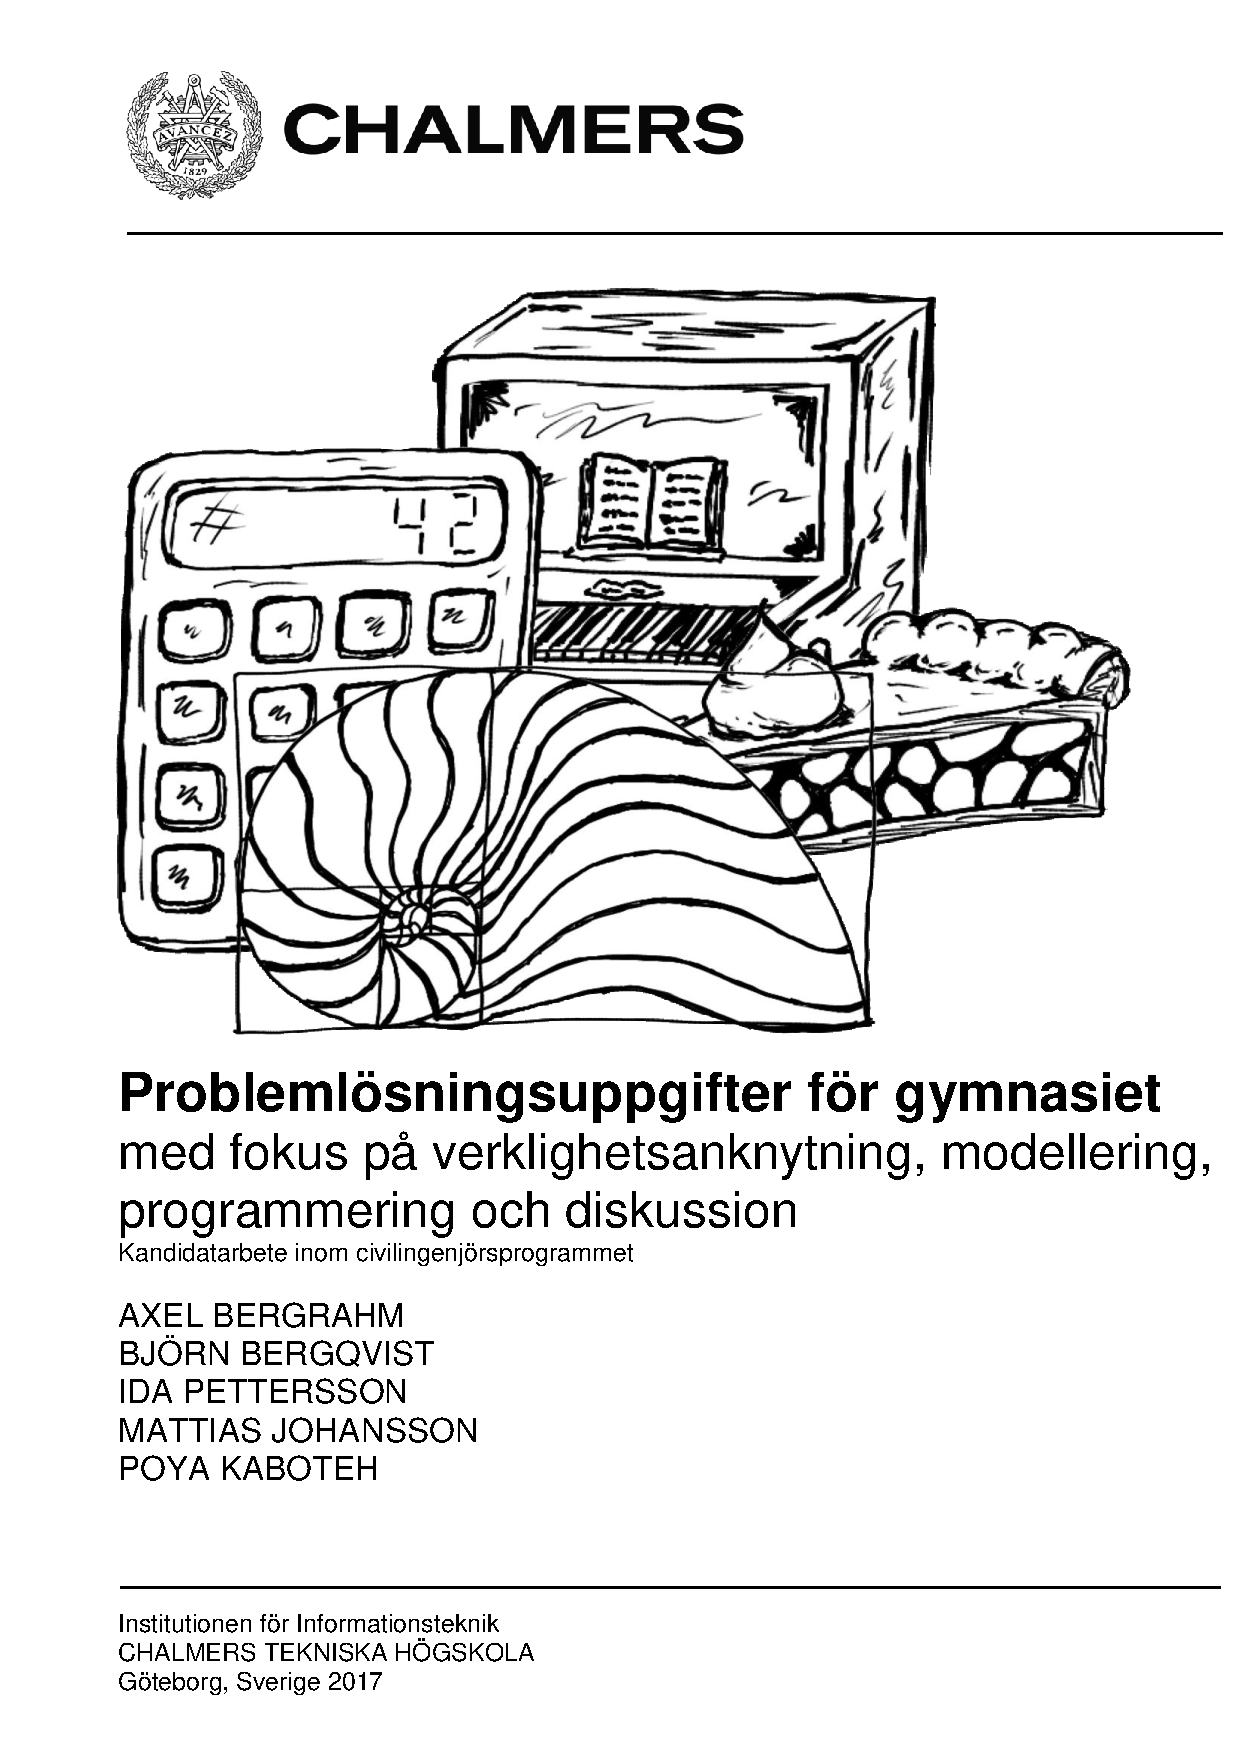
\includepdf{Figures/Framsida.pdf}
%Förslag på ny titel
% Titel: Problemlösningsuppgifter för gymnasiet
%Undertitel: med fokus på verklighetsanknytning, modellering, programmering och diskussion
% 

\pagenumbering{gobble}

\newpage

\renewcommand\abstractname{Sammandrag}\begin{abstract}
\noindent \textcolor{Mahogany}{Matematik är ett kärnämne i skolan idag, och anses av de flesta mycket viktigt. Samtidigt är det en vanlig uppfattning att det är svårt, tråkigt och oanvändbart. Med detta projekt vill vi underlätta för lärare att arbeta med problemlösning genom att införa nya typer av matematiska problem för gymnasieskolan,} 
\textcolor{green}{då vår undersökning visade att $91\%$ av gymnasielärare angav att de arbetade med problemlösning, men $42\%$ angav att de hade svårt att hitta bra problem.}
\textcolor{Mahogany}{Huvudsyftet med detta projekt har därför varit att utforma problem för att hjälpa dessa lärare. Problemen är öppna, verklighetsanknutna, ger underlag för diskussion, och ska framför allt ge känslan av att matematik är användbart. Eftersom programmering snart ska införas i skolmatematiken är även en del av problemen konstruerade för att förbereda inför det.}
\textcolor{lila}{Till problemen följer även ett förslag på en komplett lektionsplanering och allt presenteras på en användarvänlig hemsida som ger enkel tillgång för alla lärare som är intresserade.}
\textcolor{green}{De skapade problemen testades även på gymnasieskolor vilket visade att av de 26 svarande ansåg $80\%$ att de lärde sig något och $75\%$ uttryckte på något sätt att problemet var roligt eller meningsfullt. Alla lärare var också nöjda med det problem de testat och ansåg att den information som följde med dem gjorde dem enkla att sätta sig in i.}

% \textcolor{green}{Vår slutsats blev att lärare idag vill inkludera mer problemlösning i undervisningen, men att det inte är lätt att hitta bra problem, samtidigt som en del har tidsbrist. Trots att vi inte lyckades testa problemen i så många klasser som vi hade önskat, så var lärarna och de flesta av eleverna som testade problemen nöjda.}
\end{abstract}

\newpage

\renewcommand\abstractname{Abstract}
\begin{abstract} 
\textcolor{WildStrawberry}{
    DIBS!!!!
}
\end{abstract}

\newpage
 
\tableofcontents

\newpage
\pagenumbering{arabic}

%\section*{Mall med idéer, fyll gärna på mer}
%    \section{Introduktion}

    \subsection{Matematikundervisningen idag}
    
    \subsection{Förändringar under senare år}
        Här kan man ta upp de förändringar som genomförts hyfsat nyligen: 
        \begin{itemize}
            \item Det arbete som lagts på att införa mer problemlösning och modellering
                \subitem Ändrar i kursplanerna
                \subitem Mattelyftet
            \item Den nya ändringen med programmering
        \end{itemize}
        Man kan avsluta med en diskussion om att förändringarna tar mycket tid och energi m.m. och vad vårat arbete kan göra för att hjälpa till här.
        
\section{Teori}
    Teori om den pedagogik vi använder:
    \begin{itemize}
        \item Diskussioner och kommunikation inom matematik  %Björn
        \item Arbete i grupp? Olika gruppstorlekar? Fördelar/nackdelar? %Björn
        \item Programmering och matematik
    \end{itemize}

\section{Metod}
    \subsection{Skapandet av problemen}
        Hur vi har tänkt

    \subsection{Hemsidan}
    
\section{Resultat}
    \subsection{Problemen}
        På något sätt berätta om (ev. bara några av) de problem vi har skapat.
    
    \subsection{Hemsidan}

\section{Utfall}
    Här kommer svaren på enkäterna (förhoppningsvis)

\section{Diskussion}

\section{Slutsats}


% \section{Bakgrund}
%     \label{sec:Bakgrund}
%      \textcolor{lila}{Avsnittet introducerar projektet, samt de bakomliggande problem som fått oss att vilja sätt oss in i ämnet.}
    
    \section{Matematikundervisning nu och då}
        \textcolor{lila}{Matematik är en av de största delarna i skolan i Sverige idag, vilket bland annat visar sig genom att matematiken är kärnämne i både grundskolan och gymnasiet. Trots det är det ett ämne som många elever blir stressade över, och som ofta framställs som svårt, tråkigt, oanvändbart och abstrakt \cite{Ignacio&Barona}. En vanlig uppfattning verkar också vara att matematik är ett ämne som bara ett fåtal kan bli bra på \cite{Skolverket03} och ett ständigt återkommande inslag i media är det faktum att matematikkunskapen i Sverige har gått ner \cite{CompareOECD}. Men hur ser undervisningen ut idag? Vad kan man ändra för att förbättra dessa resultat?}


        
    \subsection{Traditionell matematikundervisning}
        \textcolor{lila}{Den så kallade traditionella undervisningsmetoden består av två delar: \textsl{genomgång} och \textsl{egen räkning} \cite{traditionellMatte}. Det innebär att lektionen börjar med att läraren står framme vid tavlan och går igenom ny teori varefter varje elev individuellt får träna på detta med hjälp av ett stort antal likartade uppgifter. Därefter kan eleverna kontrollera om de gjort rätt genom att jämföra svaret med facit, och därefter gå vidare. Om man får rätt svar på alla uppgifter anser man sig ha gjort det man ska utan att nödvändigtvis ha förstått teorin. Därefter upprepas samma procedur med ett nytt begrepp i centrum.} 
    
\textcolor{lila}{Med den här metoden lär sig eleverna olika matematiska begrepp och metoder, men först efter att det specifika begreppet eller metoden just presenterats. På det faktiska provet, när de själva måste ta reda på vilken metod som ska användas i varje uppgift, blir det betydligt svårare \cite{TheElephant}.}
\textcolor{WildStrawberry}{
    Just på grund av detta så tar man ett steg ifrån verklighetskopplingen och användbarheten av matematiken. När applikationen av teorin blir mekanisk istället för modellerande så tappar teorin syftet och blir mer av ett verktyg för att få ut rätt svar från en fråga. Fokus blir att man utnyttjar korrekt formel och snabbt får feedback från facit, eller andra hjälpmedel, om man fått rätt svar istället för att förstå problemet och dess underliggande moment för vad dem faktiskt innebär. }
    
    \subsection{Förändringar i matematikundervisningen}
        %Förändringar i matematikundervisningen

\textcolor{lila}{Den traditionella undervisningen var länge den som mer eller mindre uteslutande användes i Sverige, särskilt i högre åldrar. På senare år har man dock börjat att aktivt se över hur undervisningsmetoden skulle kunna förbättras.}

\textcolor{lila}{År 2011 infördes en ny och uppdaterad kursplan för gymnasiet, GY11, som bland annat påverkade matematiken. Jämfört med de tidigare kursplanerna från 2000 fanns det ett antal viktiga ändringar som gällde alla de olika matematikkurserna. %Ej nytt stycke!
Dels lägger de nya kursplanerna mer fokus på att kurserna ska anpassas efter varje program och inriktning. På så sätt plockas begreppet ''verklighetsanknytning'' upp på ett tydligare sätt. Man ska alltså lära sig hur matematik kan användas i vardagssammanhang som t.ex för att betala räkningar, men även i mer specifika sammanhang beroende på vad du kan behöva i yrkeslivet alternativt vidareutbildningen efter gymnasiet. 
En annan viktig ändring tar upp problemlösning. Detta har ingått även tidigare, men då bara som ett mål utöver de övriga. Nu ska det även användas som medel för inlärning av de andra målen. Kursplanen poängterar nu också att undervisningen ska varieras och innehålla undersökande aktiviteter. \cite{GY00-GY11}}

\textcolor{lila}{För att dessa förändringar ska kunna implementeras på ett så bra sätt som möjligt har man också gjort en stor satsning genom att utbilda alla lärare. Detta har gjorts genom \textsl{Matematiklyftet}, som är en kompetensutveckling i didaktik för lärare. Här belyses den kommunicerande, reflekterande och undersökande delen av matematiken. \cite{Nämnaren}}
            
\textcolor{lila}{Problemlösning är alltså ett mycket aktuellt ämne, som man lägger mycket resurser på att införa i matematikundervisningen. Det är dock en mycket stor förändring att genomföra, och det tar därför tid. Många lärare tycker också att det är svårt att hinna med problemlösning vid sidan av det material som redan ska täckas enligt kursplanen \cite{2016Senare}. Även de lärare som arbetar aktivt med att införa mer problemlösning stöter på problem. Kanske är det för att flesta elever är vana vid den traditionella undervisningen. Eleverna förväntar sig då att lärarna ska tala om precis hur man ska göra och vad som är rätt och fel. De gamla vanorna kan alltså sitta djupt hos både elever och lärare, och vara svåra att ändra.}

\textcolor{lila}{I mars i år (2017) beslutades också att skolan ska verka för att stärka elevernas digitala kompetens \cite{regeringen}. För gymnasiematematiken innebär detta att användingen av digitala verktyg ska bli mer central och programmering ska användas för att lösa matematiska problem \cite{itiskolan}. Även här ska det genomföras fortbildning av lärare \cite{prog_utbildning}.}
            
\textcolor{lila}{Vi har pratat med lärare som saknat tillräcklig hjälp i den här övergången till GY11. Trots den stora satsningen Matematiklyftet, där lärare utbildades om nya tankesätt kring matematikundervisning, så är det svårt att införa problemlösning i en klass som inte arbetat med det tidigare. Det finns gott om bra uppgifter, men det saknas hjälp med \emph{hur} man lär ut problemlösning från början. 
Ett rimligt antagande är att den kommande övergången, till att införa mer programmering och andra digitala verktyg i matematiken, också den kommer bli svår och ta lång tid att genomföra.}
%Ev. avsluta med något mer positivt, t.ecx hur vårt arbete kan hjälpa till
        \label{sec:Forandringar}
        
    \subsection{Verklighetsanknytning i matematiken}
        \textcolor{lila}{En vanlig uppfattning är att det finns för lite verklighetsanknytning i matematiken som lärs ut idag \cite{TheElephant}. Mot denna bakgrund är det lätt att förstå att elever kan tolka ämnet som onödigt och irrelevant, vilket förklarar varför det är så viktigt att eleverna upplever uppgifterna som relevanta.}

\textcolor{lila}{Detta är ett faktum som många kursboksförfattare tagit fasta på, men tyvärr uppnår dessa försök inte alltid målet. Ofta känns den så kallade verklighetsanknytningen forcerad, och det blir snarare dåligt förklädda standarduppgifter än faktiska problem som man kan föreställa sig att någon skulle vilja lösa. Detta riskerar att ge eleverna en känsla av att matematik inte är användbart, eftersom de får se så få exempel från dess verkliga användningsområden.
I vissa fall har man också tänkt för mycket på att den relevanta matematiken ska finnas med i uppgiften, vilket kan leda till att rimligheten blir lidande. Jo Boaler beskriver det som att eleverna inser att det finns ett speciellt ''matteland'', där det vanliga sunda förnuftet inte längre gäller \cite{TheElephant}.}
    
\textcolor{lila}{De textuppgifter som skrivs  i kursböcker med avsikt att införa en verklighetsanknytning kan också enligt vår erfarenhet i många fall brytas ner till standardproblem enbart genom att plocka ut siffrorna ur texten. På så sätt kan man också ofta bortse från den verklighetsanknytning som eventuellt finns i uppgifterna.}

\textcolor{lila}{Det verkar alltså vara viktigt med verkligehtsanknytning i matematiken, så att eleverna kan relatera till uppgiften och få känslan av att matematik är viktigt och användbart.} \textcolor{Mahogany}{Dock framhäver Lockhart i sin \textsl{A Mathematician's Lament} \cite{lockhart} behovet av att elever ska få utforska matematiken och att man ska försöka underbygga deras fantasi, snarare än att låsa alla problem vid verklighetsanknytning. Alltså bör uppgifter med verklighetsanknytning inte bara framhäva att matematik är användbart i det verkliga livet, utan även få eleven att känna att den är användbar.}
        
    \subsection{Matematikundervisningen idag}
        \textcolor{WildStrawberry}{
    Den svenska matematikundervisning innefattar i stora drag att en lärare lär ut ett eller flera teoretiska begrepp inför sin klass och sedan ska klassen repetera dessa nya begrepp tills det sitter i muskelminnet. Repetitionen i sin tur, kommer troligtvis innebära att eleven sitter med en lärobok som har en mängd definierade uppgifter där den nya teorin ska appliceras. Detta moment kommer att hamna i en sluten loop tills det är dags för det stora provet där man testar alla begrepp man tidigare gått igenom.
}

%ny rubrik? problemet?
%\textcolor{WildStrawberry}{
 %   Problemet med denna typen av undervisning är att eleven inte behöver känna igen det underliggande problemet, eleven kommer undan med att memorera hur en formel ser ut – utan att nödvändigtvis behöva förstå vad formeln gör. Inte för att testa förmågan att memorera saker är dåligt, men just på grund av detta så tar man ett steg ifrån verklighetskopplingen och användbarheten av matematiken. När applikationen av teorin blir mekanisk istället för modellerande så tappar teorin syftet och blir mer av ett verktyg för att få ut rätt svar från en fråga. Fokus blir att man utnyttjar korrekt formel och snabbt får feedback från facit, eller andra hjälpmedel, om man fått rätt svar istället för att förstå problemet och dess underliggande moment för vad dem faktiskt innebär. }


%vad matematiken & skola bör lära ut

% från intervju med Gymnasieelev när ställd frågan "blir ni skolade på hur man löser problem eller är problemlösningen ett vanligt matteproblem som är maskerat i text?": 
%" Mestadels det senare, vi gör problemlösningen i matten så man ska försöka hitta den användbara infon och lösa matteproblemet. Jag tar lite svårare matte men samma kurs som andra så min grupp får lite mer roliga problem där man måste använda logik i kombination med algebraisk matte...

% Men generellt så löser man mest maskerade matte problem"

\textcolor{WildStrawberry}{
    Enligt den nya läroplanen för matematik, som infördes 2011, så ska matematiken beröra problemlösning på så vis att man ska lära sig behärska sunt resonemang och logik. Eleven ska kunna bemöta uppställda situationer med metodik och kunna modellera en lösning från given information. Givetvis låter detta bra, men vad har egentligen ändrats - Från vår undersökning så får elever uppgifter, precis som i läroboken, maskerade i en kort saga som ska simulera ett problem. Reglerna är ofta tydliga och tanken är att man hittar siffrorna i texten och använder korrekt formel som man fått på undervisningen. 
}

%(citat från intervju? hittas i .tex filen ovanför stycket).
% HEEEJ :D ändra precis som du könner är swag! jag bara får ut något på papper just nu :)
% Haha, det är bra att du skriver! :D Tänkte bara hjälpa till när jag såg det och kunde :)
% Super! :D All hjälp är toppen, tror du jag tänker rätt på denna sektion? den är ju mycket lik den om traditionell skola
% Ja... Det är jag lite osäker på... Funderar på om det inte är bättre att du försöker lägga in delar av det du skrivit i det stycket... Det är ju också svårt att påstå saker utan källor, så det måste vi försöka vara noga med. 
% AA exakt! Men på sätt och vis har vi en "intervju" med en duktig matte-student. Som är en källa. Dock en källa 
% - intJeo a,l ol skoor.
% wow :D

% Det är nog också mer relevant till "matematiken idag". Det existerar en bekvämlighetsfaktor just på grund av tiden är bristande och därför är det najs att använda sig av färdiga problem som inte har mycket tanke bakom sig. - Eleven får övning och "problemlösning (läsförståelse)"

% :( 
% okej <3 <3<3<3<3 till synes borta :smirk:
% Haha, förlåt xp
% Tänket bara säga att vi ju kan använda det som att vi vet att det händer, men inte som att det alltid är så. Vi kan också gå in mer på att det är svårt att hinna med, och ta in lite mer från planeringsrapporten. Precis, eller inte från lärarnas håll i alla fall ;)
% Ska vi ta bort detta nu kanske :p
%Fixade! ;) Inte helt borta i alla fall!

%Här kommer några bra dåliga problemlösningsuppgifter ifrån \cite{matte5000} - MVH Björn

%Följande är en a uppgift, dvs en lätt uppgift:
\begin{displayquote}
\textcolor{turkos}{Marcus läser en bok som innehåller 420 sidor. Mellan kl 19.45 och 20.15 läser han 14 sidor. \\
Hur lång tid tar det att lösa hela boken?}
\end{displayquote}

%Svar

%Detta är en b-uppgift
\begin{displayquote}
\textcolor{turkos}{Jonas kör sin bil samma sträcka varje dag. Sträckan är en mil och Jonas brukar köra med hastigheten 90 $km/h$ en dag kör han sträckan med 100 $km/h$. \\
Hur många sekunder ''tjänar'' Jonas på det?}
\end{displayquote}

%Svar

%Följande två uppgifter är c-uppgifter, dvs de svåraste. 

\begin{displayquote}
\textcolor{turkos}{Vilket tal är x?\\
\( 2*5^x + 3*5^x = 25^{12} \)}
\end{displayquote}

%Svar

\begin{displayquote}
\textcolor{turkos}{En sandstrand är 2km lång, 30 m bred och 3 m djup. \\
Vi antar att ett sandkort ryms inom ett kubiskt område med sidan 0,2 mm.\\
Hur många sandkorn finns på stranden?}
\end{displayquote}

%Svar

%Samtliga fyra uppgifter har tagits från delkapitel 1.4 Problemlösning, som är del av 1 Aritmetik - Om tal. Finns liknande uppgifter i kapitlen om 2.2 Procentuellea förändringar och 3.2 Linjära ekvationer och olikheter. Dock saknas helt uppgifter om problemlösning för Geometri, Sannolikhetslära och statistik, samt Grafer och funktioner. 
        
    \subsection{Gruppindelning}
        \label{sec:Gruppindelning}
        \textcolor{turkos} {Det är vanligt att dela upp elever efter hur snabbt de anses lösa uppgifter. Elever som löser uppgifter snabbt grupperas med andra elever som löser uppgifter ungefär lika snabbt, och det samma gäller elever som anses lösa uppgifter långsamt och en grupp för elever som ligger mellan de två andra grupperna \cite{Skolverket03}. }

        
\section{Första enkäten}
    \subsection{Hur ser matematikundervisningen ut?}

\textcolor{lila}{Här löd frågeställningen "Uppskatta ungefär hur många procent av lektionstiden som spenderas på följande:" och därefter följde förslag på vad man kan göra på en lektion, samt en punkt för "Övrigt" där man även fick specificera vad detta innebar. Resultatet av detta visas nedan (just nu i tabeller, men detta ska överföras till cirkeldiagram)}

\begin{table}
\caption{Genomgång med hela klassen}
\centering
\begin{tabular}{||r|r|r||} \hline\hline
\emph{Andel lektionstid (\%)} & \emph{Antal (st)} & \emph{Procentandel av de svarande (\%)} \\ \hline
\hline
0 & 0 & 0 \\ \hline
1-10 & 2 & 4,3 \\ \hline
11-20 & 11 & 23,4 \\ \hline
21-30 & 26 & 55,3 \\ \hline
31-40 & 7 & 14,9 \\ \hline
41-50 & 0 & 0 \\ \hline
51-60 & 1 & 2,1 \\ \hline
61-70 & 0 & 0 \\ \hline\hline
\end{tabular}
\label{table:Genomgang}
\end{table}


\begin{table}
\caption{Egen räkning i boken}
\centering
\begin{tabular}{||r|r|r||} \hline\hline
\emph{Andel lektionstid (\%)} & \emph{Antal (st)} & \emph{Procentandel av de svarande (\%)} \\ \hline
\hline
0 & 0 & 0 \\ \hline
1-10 & 1 & 2,1 \\ \hline
11-20 & 5 & 10,6 \\ \hline
21-30 & 11 & 23,4 \\ \hline
31-40 & 14 & 29,8 \\ \hline
41-50 & 10 & 21,3 \\ \hline
51-60 & 2 & 4,3 \\ \hline
61-70 & 4 & 8,5 \\ \hline\hline
\end{tabular}
\label{table:Rakning}
\end{table}

\begin{table}
\caption{Att eleverna diskuterar med varandra och arbetar tillsammans}
\centering
\begin{tabular}{||r|r|r||} \hline\hline
\emph{Andel lektionstid (\%)} & \emph{Antal (st)} & \emph{Procentandel av de svarande (\%)} \\ \hline
\hline
0 & 2 & 4,3 \\ \hline
1-10 & 14 & 30 \\ \hline
11-20 & 10 & 21,3 \\ \hline
21-30 & 17 & 36,2 \\ \hline
31-40 & 4 & 8,5 \\ \hline
41-50 & 0 & 0 \\ \hline
51-60 & 0 & 0 \\ \hline
61-70 & 0 & 0 \\ \hline\hline
\end{tabular}
\label{table:Diskussion}
\end{table}

\begin{table}
\caption{Uppföljning reflektion med hela klassen}
\centering
\begin{tabular}{||r|r|r||} \hline\hline
\emph{Andel lektionstid (\%)} & \emph{Antal (st)} & \emph{Procentandel av de svarande (\%)} \\ \hline
\hline
0 & 3 & 6,4 \\ \hline
1-10 & 25 & 53,2 \\ \hline
11-20 & 11 & 23,4 \\ \hline
21-30 & 19 & 40,4 \\ \hline
31-40 & 0 & 0 \\ \hline
41-50 & 0 & 0 \\ \hline
51-60 & 0 & 0 \\ \hline
61-70 & 0 & 0 \\ \hline\hline
\end{tabular}
\label{table:Uppfoljning}
\end{table}

\begin{table}
\caption{Övrigt}
\centering
\begin{tabular}{||r|r|r||} \hline\hline
\emph{Andel lektionstid (\%)} & \emph{Antal (st)} & \emph{Procentandel av de svarande (\%)} \\ \hline
\hline
0 & 39 & 83,0 \\ \hline
1-10 & 5 & 10,6 \\ \hline
11-20 & 3 & 6,4 \\ \hline
21-30 & 0 & 0 \\ \hline
31-40 & 0 & 0 \\ \hline
41-50 & 0 & 0 \\ \hline
51-60 & 0 & 0 \\ \hline
61-70 & 0 & 0 \\ \hline\hline
\end{tabular}
\label{table:Ovrigt}
\end{table}

\textcolor{lila}{Genom att studera cirkeldiagrammen kan man notera att den största delen av lektionstiden används till genomgång och egen räkning. Därefter följer elevdiskussion och uppföljning, och utöver detta lägger en liten andel av lärarna även tid på andra saker. Under övrigt faller framförallt laborationer, spel, digitala quizz, redovisningar framförda av eleverna samt problemlösning.}

\textcolor{lila}{Några av lärarna kommenterade också i samband med den här frågan att de uppmuntrar eleverna att jobba tillsammans med uppgifterna i boken, och att det på så sätt blir mycket lite eget arbete, och mer diskussion mellan eleverna.}

\subsection{Vad är problemlösning för dig?}
\textcolor{lila}{Här bad vi lärarna att skriva en kort förklarande text om hur de definierar problemlösning. I de svar vi fick in kunde vi hitta några olika karatäriserande åsikter, och tittat på hur stor andel av lärarna som nämner de olika delarna. Notera att många lärare nämnde flera olika kriterier.}

\textcolor{lila}{Många lyfte fram att ett problem är \textsl{en uppgift som man på förhand inte vet hur man ska lösa, och där man får applicera känd kunskap på nya situationer}. Detta är den vanligaste definitionen, och även den vi framförallt använder i denna rapport. Hela $79\%$ hade med detta som ett kriterium i sina definitioner av problemlösning.}

\textcolor{lila}{En annan viktig faktor, som nämndes av ungefär $20\%$, var \texsl{öppna problem}. Dessa definieras av att de går att lösa på flera olika sätt, och i vissa fall även kan ge olika svar. Ett exempel på ett öppet problem är att man ska planera en pool med en viss volym, vilket självklart kan göras på en mängd olika sätt.}

\textcolor{lila}{Därefter följde två kritierer, som vardera nämndes av cirka $16\%$. Det ena var att problemlösning ska utgå från en större uppgift, vilken man måste använda flera olika metoder för att lösa. Den andra pekar på att ett problem innehåller för mycket eller för lite }
    %\newline \newline 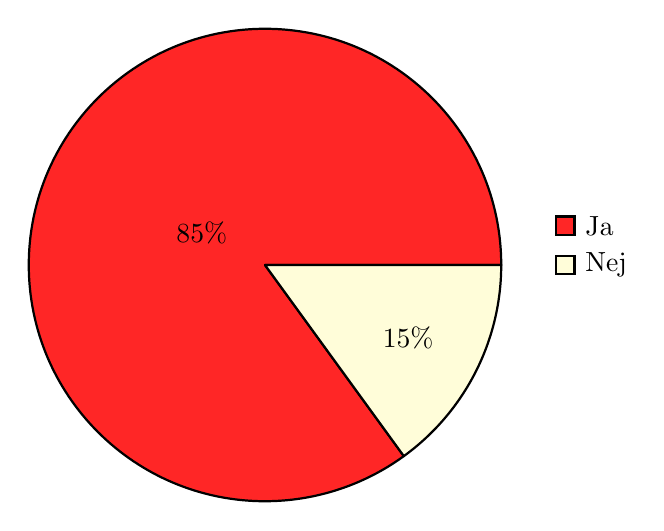
\begin{tikzpicture}
    \pie [text = legend, color={red!85, yellow!15}]{85/ Ja, 15/ Nej}
\end{tikzpicture}
    
\section{Teori}
    \label{sec:Teori}
    \input{Sections/Teori/Teori.tex}
    
    \subsection{Vad är ett problem?}
        %\textcolor{Mahogany}{Vi definierar ett problem som en uppgift som man på förhand inte vet hur man ska lösa. }

% Vad är inte problemlösning
\textcolor{WildStrawberry}{
    Komplexiteten med att definiera vad ett problem är ligger i att det existerar olika syften med vad ett problem vill få ut från den som testas. Vissa problem vill att du hittar x - kan du hitta x? Andra problem kanske inte har ett exakt svar - tillvägagångssättet när man försöker lösa problemet är det som är utvecklande. Det vi vill ta ställning för är att en ''lös ut x''-uppgift som är dekorerad i en \textit{saga} skapar inte ett intressant problem och kunde lika väl varit den vanliga ''vad är x''-övningen. 
}

% Vad är problemlösning
\textcolor{WildStrawberry}{
    Det finns en mängd olika infallsvinklar man kan ta för att definiera \textit{ett problem}. Den som testas bör behöva fundera på vad som är viktigt i en given situation och skapa egen modellering av verkligheten. Ett problem bör skapa ett behov för teorin som kan appliceras och därav förhoppningsvis härleda för en djupare förståelse till varför teorin fungerar. När man fått fundera på hur man \textit{kan} gå till väga för att lösa problem innan man får underlaget så binder man en starkare koppling till materialet och bör därför komma ihåg det bättre\todo{källa}. Men vi vill definiera att \textit{ett problem} är en form av uppgift där man får arbeta med en situation eller uppställning som man inte kan svaret till på förhand.
}


    \textcolor{lila}{Denna definition gör det på sätt och vis mycket svårt att skapa ett problem, eftersom den innebär att en uppgift som är ett problem för en person, kan vara en ren standarduppgift för någon annan. Definitionen innebär också att problemlösning är ett mycket brett område. Nedan presenteras några viktiga delar som, tillsammans eller var och en för sig, kan lyftas fram i ett bra problem.}
    
    \textcolor{lila}{Till att börja med kräver problemlösning ett \textsl{undersökande arbetssätt}. det handlar om att analysera problemet och bryta ner det i mindre delar, och därefter hantera varje del var för sig. Ofta måste man prova sig fram med olika lösningsmetoder innan man hittar en som fungerar.}
        
    \textcolor{lila}{En vanlig form av problemlösning är genom att använda \textsl{öppna problem}. Det innebär ett  problem till vilket det finns flera olika möjliga lösningsgångar för att hitta ett svar, och detta svar behöver inte heller vara unikt utan kan variera beroende på vilka antaganden som gjorts.}

    \textcolor{lila}{En annan viktig del är att kunna översätta ett problem i \textsl{matematiska modeller}. Detta är en nyttig förmåga att besitta i många olika sammanhang, även i arbetslivet~\cite{TheElephant}. Det är också minst lika viktigt att kunna granska en modell med kritisk blick, och fundera på i vilka sammanhang den gäller och när den leder till orimliga resultat.}
        
    \subsection{Diskussioner och kommunikation inom matematik}
        \textcolor{turkos} {
Givande diskussioner kan få elever att inse att det är tillåtet att ha egna idéer och tankar kring matematik, ett ämne som annars ofta upplevs handla om att följa regler. När elever diskuterar problem med varandra så lär de av varandra, och kan ofta uttrycka sig på ett sätt som kan göra det lättare för dem att förstå än vad ofta läraren kan. \cite{TheElephant}
}

\textcolor{turkos} {Faktum är att diskussion är så viktigt för bra problemlösning att Hagland m.fl. skriver, i deras bok Rika matematiska problem, att den viktigaste skillnaden mellan ett vanligt problem och vad de kallar ett rikt problem är att det rika problemet leder till diskussion \cite{RikaProblem}. Även Skolverket lyfter att matematikundervisning där elevers egna lösningstratergier diskuteras leder till mycket positiva resultat och ökar elevers lust att lära\cite{Skolverket03}.}

\textcolor{turkos}{I Rika matematiska problem beskrivs även vikten av ha en avslutande klassdiskussion \cite{RikaProblem}. Anledningen till att boken lägger vikt vid diskussion just på slutet är att alla elever tid att jobba med problemet, även om alla kanske inte har löst det, och kan därmed bidra till diskussionen. Även läraren har haft möjlighet att bilda sig en uppfattning om vilka metoder eleverna har använt för att lösa problemen och kan därmed leda diskussionen och ta upp intressanta idéer som uppstått i klassen och lyfta dem till resterande elever.}

\textcolor{turkos} {
Ett land som tas upp som ett exempel på god matematikundervisning av både Skolverket och Boaler är Japan \cite{TheElephant}\cite{Skolverket03}. Skolverket beskriver hur det i Japan läggs stor vikt vid att efter eleverna löst ett problem så ska de dela med sig utav sina lösningar och diskutera dem med varandra. Där används diskussionen som en utgångspunkt för att läraren ska kunna lyfta viktiga aspekter ur deras lösningar och tillvägagångssätt.}

% Rika problem är problem som leder till diskussion

% Ger chans att lyfta sina egna idéer och utveckla dem. 

% Diskussion leder till öka lust att lära. 

% Japanska skolan lägger fokus på diskussion och lyfts som ett föredöme av både skolverket och Jo Boaler 

% Tar upp strukturen med diskussion före och efter elever får lösa problemet. 


% Skriv något om att det är bra att reflektera efter man har gjort en uppgift. 
        
    \subsection{Arbeta i grupp}
        \textcolor{turkos} {
Att låta elever arbeta med problemlösning i små grupper om två till fyra personer leder till att varje elev ges möjlighet att diskutera och reflektera angående problemet. Eleverna får prata om sina idéer till lösningar, lyssna på andra elevers idéer, samt även ges möjlighet att fråga, kritisera och bemöta kritik på ett positivt sätt. När eleverna får förklara sina tankar leder det till ökad matematiksförståelse. \cite{RikaProblem}
}

\textcolor{turkos} {
Som tidigare nämnts i \ref{sec:Gruppindelning} är det vanligt att skolor delar in elever i grupper efter deras matematikfärdigheter, dock hävdar både Boaler \cite{TheElephant} och Rika matematiska problem \cite{RikaProblem} att det är bättre med heterogena grupper vad det gäller matematikkunskap. I blandade grupper där man arbetar efter metoder anpassade för dem får elever lära av varandra vilket leder till ett mer rättvist klassrum enligt Boaler \cite{TheElephant}. 
}

\textcolor{turkos} {
Rika matematiska problem rekommenderar att läraren blandar medelpresterande elever med högepresterande eller lågpresterande elever när man gör gruppindelningen, men varnar samtidigt för att inte göra grupperna extremt homogena eller heterogena\cite{RikaProblem}.
}

% I blandade grupper hjälper elever varandra vilket leder till fina ord som equality och allt blir bättre - Jo Boaler

% Även Rikaproblem rekommenderar att man blandar medelpresterande elever med högepresterande eller lågpresterande elever när man gör grupp indelningen, men varnar samtidigt för att inte göra grupperna extremt homogena eller heterogena. 


\textcolor{turkos} {
En negativ aspekt med grupparbete är att vissa elever kan bli sittande passivt medan resten av gruppen löser uppgiften åt dem\cite{RikaProblem}. Detta problemet kan rimligen antas bli värre ju större gruppen blir. 
}

%Bygga en rödtråd till förra kapitlet genom Japanska skolan. 



% Problemlösning i grupp anses vara roligare än vanliga mattelektion - Skolverket

% Saknas något om olika gruppstorlekar, samt nackdelar

% En studie visar att 2 är bättre än 1 förrutom för de allra bästa eleverna där det är ungefär lika bra, men 3-5 är strängt bättre. Den säger även att testpersonerna hade något roligare när det arbetade individuellt.

%Negativt - Om man börjar med grupparbete så kan vissa elever bli sittande passivt medan resten av gruppen löser uppgiften åt dem. - Rikaproblem



% Grupper bör ligga på 2-4 elever, eftersom det i en sådan grupp ger alla elever möjlighet att delta i diskussioner - Rika problem 

% Gruppering efter färdigheter är vanligt, enligt skolverket. 
        
    \subsection{Programmering och matematik}
        \textcolor{Mahogany}{Att lära sig programmera är att inte bara lära sig ett programmeringsspråks syntax, det är framför allt att kunna bryta ner ett problem i mindre delar, också kallat subrutiner, och definiera tydliga steg för hur man genomför dessa. Att få den träning och tillslut färdighet för detta gör att man med större sannolikhet kommer att kunna bemöta ett nytt problem på ett mer systematiskt och rationellt sätt.}

\textcolor{Mahogany}{Eftersom en dator behöver exakta instruktioner utan egen förmåga att tolka vad som är rätt och fel så är det viktigt att man är tydlig med vad man verkligen menar att ett program ska göra. Vad en dator däremot är bra på är att utföra dessa instruktioner på väldigt kort tid. Detta ger ett väldigt kraftfullt verktyg för många saker, faktum är att detta så kallade verktyg används i så stor utsträckning att vårt moderna samhälle är beroende av det. Det kan handla om att kunna betala sina räkningar på internetbanken till att hitta ett lunchställe i en ny stad med hjälp av sökmotorer.}

\textcolor{Mahogany}{Vikten av att lära sig programmering är inte bara att det är en kunskap som är mer och mer efterfrågad, men för att det är en möjlighet för elever att med relativt fria tyglar få syssla med problemlösning, något som man har väldigt stor nytta av i matematik\cite{TheElephant}, och som matematik i stor utsträckning även går ut på. Som vi nämnt i \ref{sec:Forandringar} så kommer programmering från och med i år (2017) att ingå i kursplanen för gymnasiematematik, vilket gör det väldigt aktuellt att inkludera matematikrelaterade programmeringsuppgifter i vårt projekt, och de flesta av de programmeringsuppgifter som vi tagit fram har en tydlig koppling mellan de två ämnena.}
        
    \subsection{Info om React?}
        
\section{Syfte}
    \subsection{''Mattedelen''}
    (Skriva om syftet med problemen, även varför vi riktar oss mot just gymnasiet.)
    \subsection{Hemsidans utvecklingsmiljö}
        \textcolor{Mahogany}{Hemsidan är ett sätt att förmedla de problem som vi utformat till fler än de som vi testar problemen med genom att göra det mer lättillgängligt att ta del av problemen. Med hjälp av denna kan vi ge lärare möjligheten att ta del av våra problem när de vill och känner att de har tid över. Det hjälper oss också att få spridning på problemen som vi utformat. Kanske tyckte de att problemen var givande och delar med sig av sidan till en kollega, som kanske i sin tur gör samma sak. I slutändan så hoppas vi helt enkelt att så många som möjligt kan ha hjälp av de problem som vi utformat.}

\textcolor{Mahogany}{Hemsidan är också det som kommer att leva kvar efter projektet, så vi har valt att inkludera en kort beskrivning om oss och vårt arbete, samt en liten informativ text till lärare med vad vi vill uppnå med våra problem och hur vi tänkt att de bör utföras.}

\section{Metod}

    \subsection{Skapandet av problemen}
        \textcolor{lila}{De problem som har skapats har som tidigare nämnts konstruerats med målet att öka andelen problemlösning i gymnasiet. För att uppnå detta har vi vid skapandet av problemen utgått från ett antal riktlinjer, där en eller flera av dessa belyses i varje problem.}

\textcolor{lila}{Den första, och kanske viktigaste, riktlinjen är att problemen ska leda till ett \textsl{undersökande arbetssätt}, se avsnitt~\ref{sec:problemdef}. I samma avsnitt diskuteras även \textsl{öppna problem}, som också var en bakomliggande tanke för många av problemen. Vi har även skapat problemen med avsikt att träna eleverna på \textsl{modellering} och \textsl{programmering}, vilka tas upp i avsnitt \ref{sec:problemdef} respektive \ref{sec:ProgrammeringOchMatematik}. \textsl{Verklighetsanknytning} ska också enligt avsnitt~\ref{sec:Verklighetsanknytning} finnas med i flera av problemen. Alla problemen har också konstruerats för att vara \textsl{rika problem}, se avsnitt~\ref{sec:Diskussion} som kan leda till en givande diskussion.}

\textcolor{lila}{Med detta som underlag har vi skapat olika problem. Vi har tagit inspiration från våra egna erfarenheter från hela vår skolgång, inklusive universitetet, samt från en mängd olika böcker, som nämns i samband med respektive problem. Utifrån vår grundidé har vi därefter arbetat oss vidare för att skapa ett problem som passar gymnasieelever. På så sätt har vi tagit fram problem som alla har tre gemensamma delar: \textsl{Introduktion}, \textsl{Genomförande} och \textsl{Diskussion}.}

\textcolor{lila}{I introduktionen presenteras problemet, och i vissa fall ingår där ett antal frågor att diskutera innan man börjar räkna på problemet. Själva problemet genomförs i grupper om två, och därefter kommer diskussionen. Denna börjar i vissa fall med att man går ihop i lite större grupper och presenterar och diskuterar sina lösningar av problemet, förklara varför man gjort som man gjort och jämföra eventuella olika lösningsgångar. Avslutningsvis diskuterar klassen problemet tillsammans, eventuellt med hjälp av våra föreslagna diskussionsfrågor. Vikten av att diskutera  problemet ordentligt presenteras i avsnitt~\ref{sec:Diskussion}.} 

\textcolor{lila}{Till varje problem följer också \textsl{Information till läraren}, med information om problemets mål samt eventuella förkunskaper och material som behövs. Det finns också \textsl{Ytterligare information}. Dit kan höra förslag på hur problemet kan introduceras, bakgrundsinformation som kan vara bra för läraren att repetera innan problemet genomförs med klassen samt tankar om vilka frågor som skulle kunna dyka upp vid diskussionerna och hur dessa kan hanteras. Till många problem finns också en presentation, som läraren kan välja att använda. På så sätt presenteras problemen tillsammans med en komplett lektionsplanering.}

\textcolor{lila}{Vi har även skrivit en text som förklarar tanken med våra problem. Där presenteras upplägget samt några idéer på hur man ska agera som lärare, bland annat genom att undvika att framställa ett förslag som felaktigt.}

\textcolor{lila}{De problem som ska testas har planerats för att ta ungefär 50 minuter att genomföra. Detta för att de ska kunna genomföras under en lektion på en timme, och att det ska finnas tid över att svara på utvärderingsenkäten, vilken kommer att diskuteras i kapitel~\ref{sec:testavproblemen}.}

\textcolor{Mahogany}{Metoden kring hur vi utformade problemen och vilken nivå de skulle ligga på var att vi med relativt stor frihet tog fram problem på gymnasienivå.
Den mer specifika nivån var menad att vara anpassningsbar, på det sättet att man med hjälp av fördjupningsfrågor kunde fördjupa sig inom ämnet och därmed kunna försvåra problemet om så önskas.
I det senare stadiet av projektet blev det dock viktigare att bestämma en nivå då lärare som skulle testa problemen ofta enbart undervisade på en specifik nivå. Behovet av att bestämma en nivå för problemen, alternativt anpassa problem utefter en viss nivå, blev därmed större.}
    
    \subsection{Test av problemen}

    \subsection{Hemsidan och latexponering}
        \textcolor{green}{Hemsidan utvecklades i programmeringsspråket Javascript. Fördelarna med att använda sig av ett programmeringsspråk som Javascript istället för att exempelvis bara använda HTML är att man kan designa sidan på många fler sätt och får total kontroll över sidans innehåll. Med total kontroll menas det att man skulle kunna ha annan material på webbplatsen än bara text- och bildmaterial. Det skulle kunna vara någon form av digitalt verktyg, t ex ett matematiskt problem som använder sig av en simulator. Detta kan göras med hjälp av Javascripts många olika bibliotek.}

\textcolor{green}{Biblioteket som användes för att utveckla webbplatsen var React JS. React JS är ett av de mest populära biblioteken att bygga webbplatser med i Javascript [källa]. I Reacts bibliotek finns främst verktyg för att jobba med vy-delen av en hemsida. Vill man integrera tyngre applikationer i webbsidan så finns möjligheter för det. Men om vyn är det största fokuset så är React ett mycket lämpligt val då det är väldokumenterat och gör det enkelt att bygga vidare på hemsidans design.}

    
\section{Resultat}

    \subsection{De problem som vi skapat}
    
    \subsection{Hemsidan}
        \textcolor{Mahogany}{Hemsidans design har gjorts enkel där känslan ska vara att man hela tiden är på ''en'' sida. Den består av olika problem som listas i ett rutnät på ''Problem''-sidan, innehållandes titel och bild. Klickar man på ett av problemen i rutnätet så kommer man vidare till en mer detaljerad vy över problemet med en kort beskrivande text följt av en länk till det fullständiga problemet. I många fall bifogas även en tillhörande PowerPoint, som är tänkt att underlätta utförandet. För programmeringsuppgifterna så bifogas även ett lösningsförslag skrivet i Java.}

\textcolor{Mahogany}{Hemsidan har även en startsida som designats för att kännas inbjudande och engagerande, där besökaren ges en introducerande text om vad vi arbetar med samt en knapp som tar personen direkt till problemen. Dessa kommer man givetvis också åt via menyn, skillnaden är att vi vill fånga uppmärksamheten på ett mer välkomnande sätt för den som besöker hemsidan för första gången genom att ha en knapp över en bild som illustrerar några av våra problem.}

\textcolor{Mahogany}{Till sist så inkluderas sidan ''Om oss'', som beskriver projektets arbete, samt en sida med ''Information till läraren'', vars innehåll beskrivs närmare i \ref{sec:Skapandetavproblem}.}

\section{Utfall}
    \label{sec:Utfall}
    \begin{itemize}
\item Hur problemen togs emot av lärare och elever
\item Att det fanns ett stort intresse i början av att testa uppgifterna, men att många hoppade av pga tidsbrist i samband med de nationella proven.
\end{itemize}


\section{Diskussion}

    \subsection{Hur vi kan påverka}
        % \textcolor{Mahogany}{
%     Som nämndes i avsnitt~\ref{sec:slutenkat} så var det under utvärderingen inte ovanligt att lärare kände att de inte hade tid att testa våra problem på grund av annat i kursplanen så som nationella prov. De var dock intresserade, och de flestakommenterade att problemen och uppläggen verkade bra. Vi hoppas därför att även om många lärare just nu inte kan utvärdera våra problem att vi ändå lyckats förmedla nyttan med denna typ av arbetssätt och att matematik bör handla mer om den undersökande delen som till större del bygger på diskussion och rimlighetsanalyser.
% }

\textcolor{Mahogany}{
    I \ref{sec:MerProblemlosning} så framgår det att många lärare påpekar att de anser problemlösning vara viktigt. Samtidigt känner de att de inte kan arbeta med det till den grad de skulle vilja på grund av tidsbrist, både på och inför lektionerna, och för att de inte vet hur man skulle göra det på ett bra sätt. De tyckte bland annat att det var svårt att hitta bra problem som är utmanande för hela klassen. %I utformandet av våra problem så försökte vi i någon mån att anpassa problemen efter vissa nivåer, kanske främst för testningssyften då vissa lärare uttryckte intresse av att testa problem som specifikt skulle passa in på en viss matematikkurs. Vi hade egentligen som utgångspunkt att utforma \textsl{bra} problem, utan hänsyn till vilken nivå den hamnar på. Samtidigt kan det vara bra att ta försöka få in vissa element som gör att man kan fånga upp relevant teori, eller efterfrågan av den, även om fokus fortfarande ligger på problemlösning.
}

    \textcolor{lila}{Med den fullständiga lektionsplanering som följer med hoppas vi kunna avlasta lärarna från en del av det förberedande arbete som krävs för att genomföra en problemlösningslektion, och därmed förbättra deras arbetssituation. Med den brist på lärare som råder idag är det viktigt ur ett samhällsperspektiv att spara på de resurser vi har, för att kunna utnyttja deras fulla potential genom att de får finnas till hands och handleda problemlösningen. Bristen av ren lektionstid är svårt för oss att påverka, men dels har vi även tryckt på den bevisade nyttan av problemlösning och dels hoppas vi som sagt att detta ska hjälpa med en del av de nuvarande faktorer som motverkar mer problemlösning i undervisningen.}
    
    \textcolor{lila}{Även om man arbetar hårt för att ändra matematikundervisningen, och utvecklingen enligt oss är på väg åt rätt håll, så tror vi att det finns mer som kan göras för att hjälpa den på traven. Vi vill därför arbeta för att hjälpa lärarna att få eleverna att gå från att beskriva matematiken som ''tråkig'' och ''onödig'' och istället börja använda ord som ''rolig'', ''spännande'' och ''användar''. Kanske till och med ''kreativ''.}
    
% \textcolor{Mahogany}{
%     Vi hoppas att även om det är en småskalig inverkan så kan vi fortfarande hjälpa till att förändra bilden kring matematik så att den inte ska förknippas med ord som och att elever ska känna att det är något kreativt och undersökande snarare än att handla om memorering och upprepning.}
    %\textcolor{lila}{Och även om detta bara är en liten del av den utveckling vi hoppas följer, så hoppas vi att matematikundervisningen utvecklas till en mer levande och kreativ process. I bästa fall leder detta till en ny generation av skickliga problemlösare, som kan säkra Sveriges roll i framtidens tekniska samhälle. 
%}
    
    \subsection{Vad är ett bra problem?}
        % Vi testade bara problem som utfördes under 1h
\textcolor{Mahogany}{Målet med de problem som vi utformat i projektet är att framhäva vikten av problemlösning i matematiken. Samtidigt så är också ett mål att visa hur den kan vara användbar, och att den användbarheten inte enbart existerar i ''mattelandet'', som beskrivs i \ref{sec:Verklighetsanknytning.}. Ett \textit{bra} problem bör alltså inte bara framhäva att matematik är användbart i det verkliga livet, utan att även få eleven att känna att det är användbart. Detta kan vara betydligt lättare att uppnå med programmeringsproblem, då man, utöver programmeringsspråkets syntax, inte är bunden till hur man kan lösa något av problemen. Man ges också i många fall möjligheten att själv avgränsa hur utförligt problemet ska utföras. Som exempel så har vi utformat ett problem där man ska verifiera ett personnummer, där man företrädesvis kan använda sig av den så kallade Luhn-algoritmen\cite{Luhn}. Dock så kanske det inte räcker med att enbart kontrollera med hjälp av den algoritmen. Om man kontrollerar personnummer på de i sin klass så kanske man vill kontrollera att personen inte är född på 1800-talet exempelvis!}

%Hej! :) Tänkte lägga in en massa text här, som jag tycker passar bättre i diskussionen än i metoden. Hoppas det är ok :)

% Hej! Det är ok! (-8

 %:-------) :p
 
% Ta ställning till omständigheter
\textcolor{Mahogany}{Något som är viktigt att ta ställning till när man utformar problem för gymnasiematematik är att det måste vara förenligt med övriga undervisningen. Man ska övertyga både lärare och elever att det för det första är relevant, men också att det kommer att vara mer givande än att räkna i boken. Det är också viktigt att ha som en röd tråd vad man egentligen vill att elever ska få ut av ett problem, och försöker förmedla detta på ett naturligt sätt. Är problemlösning bara något som tar tid från räkning i boken eller kan man få elever att förstå att de kan gynnas av denna typ av matematikundervisning? Ett ''bra'' problem bör rimligtvis lyfta fram den nyttan. Framför allt så bör de även vara roliga att lösa.}

% Hur bör det utföras?
\textcolor{Mahogany}{Vi har lagt ner en del tid på att informera lärare hur vi tänker att våra problem ska utföras. Detta är för att vi vill att man ska få ut så mycket som möjligt från problemen framförallt via diskussion och reflektion. Diskussionsdelen är också ett sätt för elever att våga försöka lösa ett problem som till synes kanske skulle vara avskräckande. Oavsett svårighetsgraden på problemet så anser vi att diskussionen är en viktig del i lärandet, då man får möjligheten att uttrycka sin nivå av förstående och ens kunskap testas genom att man behöver förklara det för någon annan. Samtidigt så gynnas de elever som inte kommit lika långt av att få höra hur andra tänkt, och därifrån kunna arbeta vidare själva.}

% Rimlig nivå
\textcolor{Mahogany}{En svårighet med att utveckla problem är att sätta en rimlig svårighetsgrad, speciellt med tanke på att vi under utvärderingen fick jobba med framför allt väldigt specifik tidsram. Ett sätt att konfrontera detta är att ha en tydlig grund som problemet bygger på, för att sedan möjliggöra vidareutveckling i största mån. Denna vidareutveckling handlar ofta om fördjupningsfrågor som uppmanar till diskussion, vilket kan underbygga elevernas möjlighet att få en djupare förståelse för ämnet.}
\newline

% Risken med verkliga problem
\textcolor{Mahogany}{En utmaning med att försöka anknyta matematik till något verkligt är att det finns en risk att bli krystat och samtidigt tar ifrån eleven rätten att utforska hur något kan användas i verkligheten. I ''A Mathematician's Lament'' \cite{lockhart} så framhäver Lockhart behovet av att elever ska få utforska matematiken och att man ska försöka underbygga deras fantasi istället. En utmaning med att utforma ''verkliga'' problem är att ta ställning till detta samtidigt som man vill framhäva den mångsidiga nyttan med matematiken.}

        
    \subsection{Problemlösning}
        \textcolor{Mahogany}{Från svaren på en av våra undersökningsenkäter så märkte vi att begreppet problemlösning skiljde sig markant från lärare till lärare, där vissa kände att räkning i boken var problemlösning medan andra redan tidigare hade försökt att arbeta med liknande arbetssätt som vi försöker framhäva. Problemlösning är dock inte ett helt självbeskrivande begrepp som med fördel kan förtydligas.}

\textcolor{Mahogany}{Även om problemlösning är en del av kursplanen i matematik så är det tydligt att det skiljer sig i vilken utsträckning och form det utövas. Som nämnts i \ref{sec:Forandringar} så ska problemlösning vara både ett mål och medel i undervisningen enligt kursplanen för gymnasiematematik, dessvärre så förlitar sig lärare i stor utsträckning enbart på de problem som kursboken tillhandahåller. Därtill blir den typen av problem ofta enbart extrauppgifter för de som hinner \cite{2010UndervisningenGymnasieskolan}. Det är alltså rimligt att anta att problemlösning i gymnasiematematik är bristfällig samt att lärare behöver fler verktyg och resurser för att uppnå dessa mål.}

\textcolor{Mahogany}{Vi tror att en stor del handlar om att låta elever få diskutera med varandra, men utformningen av rätt typ av problem är givetvis också viktigt. Det ska inte mynna ut till att handla om att ta ur värden och sedan applicera dessa på aktuell teori som nyss gåtts igenom. Men det gäller också att ge lärare resurserna och samtidigt utmana deras uppfattning om vad problemlösning är, för att på så sätt kunna öka andelen av vad vi ser som problemlösning.
Kanske är en stor anledning att det inte är mer problemlösning i undervisningen att lärare i olika utsträckning är osäkra på hur de ska genomföra en sådan undervisning, med en kombination av att inte ha rätt resurser. Frågan är om man uteslutande kan förlita sig på att enbart kursböckerna ska täcka denna del av kursplanen, men samtidigt krävs tid och resurser om man vill förbättra detta, något som många lärare känner att de inte har.}
    
    \subsection{Hemsida}
        \textcolor{WildStrawberry}{
    %Just att ha en plats där vem som helst kan ha åtkomst till problemen anser vi är viktigt. När möjligheten finns att kunna dela information på ett lättillgängligt sätt, då når man potentiellt ut till fler lärare som skulle vara intresserade utav att testa problemen. 
}

\textcolor{WildStrawberry}{
    %Motargumentet till att bygga en hemsida är att vi skulle kunna skicka ut PDF-filer per epost till lärare - vilket var fallet när vi testade problemen. Men potentialen för spridning blir mycket enklare med möjligheten att klistra in en länk i ett mail, chattrutor eller sociala nätverk än att först ladda ner en fil och sedan bifoga den. Tanken är att ju fler handlingar som finns i en interaktion, ju större chans är det att man missar engagemangen att dela med sig till vänner och kollegor som potentiellt skulle vilja testa.
}

\section{Slutsats}

\newpage
\begin{thebibliography}{3}
        %Skriv källa:
    %1
    \bibitem{Ignacio&Barona}
    N.G. Ignacio, L.J.B.N.a.E.G. Barona, "The Affective Domain in Mathematics Learning," i \textsl{IEJME-Mathematics Education}. [Online]. Tillgänglig: \url{http://iejme.com/makale/70}. Hämtad: 5 apr 2017.
    
    %2
    \bibitem{Skolverket03}
    Skolverket, ''Lusten att l{\"a}ra : med fokus p{\aa} matematik : nationella kvalitetsgranskningar 2001-2002'',  Skolverket, Stockholm, Skolverkets rapport, 1103-2421 ; 221, 2003
    
    %Rapportserie och nummer, volym, år. [Online]. Tillgänglig: \url{http://www.mah.se/pages/45519/lustattlara.pdf}. Hämtad: datum.
   
    % Author(s). Book title. Location: Publishing company, year, pp. 
    % http://libris.kb.se/bib/8904038?vw=full
    
    %3
    \bibitem{CompareOECD}
    “Compare your country - PISA 2015,” Compare your country by OECD. [Online]. Tillgänglig: http://www.compareyourcountry.org/pisa/country/SWE. Hämtad: Feb. 10, 2017.
    
    %4
     \bibitem{traditionellMatte}
    E. Berggren, "Traditionell skolmatematik: En studie av undervisning och lärande under en matematiklektion," examensarbete, Institutionen för datavetenskap, fysik och matematik, Linnéuniversitetet, Växjö, Sverige, 2010. [Online]. Tillgänglig: \url{http://www.diva-portal.org/smash/get/diva2:337889/FULLTEXT01.pdf}. Hämtad: 7 mars, 2017.
    
    %5
    \bibitem{TheElephant}
    J. Boaler, ''The Elephant in the Classroom: Helping Children Learn and Love Maths,'' 
    London,
    England: Souvenir Press Ltd, 
    2010. 
    
    %6
    \bibitem{Nämnaren}
    E. Silver, M. Smith, "Samtalsmiljöer," Nämnaren, nr. 1, ss. 55-59, feb. 2015. [Online]. Tillgänglig: \url{http://ncm.gu.se/pdf/namnaren/5559_15_1.pdf}. Hämtad: Apr. 4, 2017
    
    %7
    \bibitem{2016Senare}
    ''Senare matematik i gymnasieskolan (matematik 3c),'' Startsidan - Skolinspektionen. [Online]. Tillgänglig: \url{https://www.skolinspektionen.se/sv/Beslut-och-rapporter/Publikationer/Granskningsrapport/Kvalitetsgranskning/senare-matematik-i-gymnasie-skolan-matematik-3c/}. Hämtad: Feb. 10, 2017.
    
    %8
    \bibitem{2010UndervisningenGymnasieskolan}
    “Undervisningen i matematik i gymnasieskolan,” Startsidan - Skolinspektionen. [Online]. Tillgänglig: \url{https://www.skolinspektionen.se/sv/Beslut-och-rapporter/Publikationer/Granskningsrapport/Kvalitetsgranskning/------Undervisningen-i-matematik-i-gymnasieskolan/}. Hämtad: Feb. 10, 2017.
    
    %9
    \bibitem{lockhart}
    P. Lockhart, \textit{A mathematician's lament}. New York: Bellevue Literary Press, 2009.
    
    %10
    \bibitem{GY00-GY11}
    Skolverket, ''Jämförelse med kursplan 2000,'' 2011. [Online]. Tillgänglig: \url{https://www.skolverket.se/laroplaner-amnen-och-kurser/gymnasieutbildning/gymnasieskola/mat}. Hämtad: Apr. 11, 2017.
    
    %11
    \bibitem{regeringen}
    Regeringskansliet, ''Stärkt digital kompetens i läroplaner och kursplaner,'' \textsl{regeringen.se} 2017. [Online]. Tillgänglig: \url{http://www.regeringen.se/pressmeddelanden/2017/03/starkt-digital-kompetens-i-laroplaner-och-kursplaner/}. Hämtad: Apr. 11, 2017.
    
    %12
    \bibitem{itiskolan}
    ?
    M. Halápi, K.L. Rüter, ''Redovisning av uppdraget om att föreslå nationella IT-strategier för skolväsendet'', Skolverket,
    
    \url{https://www.skolverket.se/om-skolverket/publikationer/visa-enskild-publikation?_xurl_=http\%3A\%2F\%2Fwww5.skolverket.se\%2Fwtpub\%2Fws\%2Fskolbok\%2Fwpubext\%2Ftrycksak\%2FBlob\%2Fpdf3647.pdf\%3Fk\%3D3647}
    
   %13
   \bibitem{prog_utbildning}
   Skolverket, ''Tydligare om digital kompetens i läroplaner, kursplaner och ämnesplaner'', 2017. [Online]. Tillgänglig: \url{https://www.skolverket.se/skolutveckling/resurser-for-larande/itiskolan/styrdokument}. Hämtad: Apr. 11, 2017.
   
   %14
   \bibitem{RikaProblem}
    Hagland, K., Hedrén, R. and Taflin, E., \textit{Rika matematiska problem - inspiration till variation}, Malmö, Sverige, Elanders Berlings AB, 2005.
    
    %15
    \bibitem{Luhn}
    “modulus 10 - Uppslagsverk - NE.” [Online]. Tillgänglig: \url{http://www.ne.se/uppslagsverk/encyklopedi/lång/modulus-10}. 
    Hämtad: Apr. 25, 2017.
\end{thebibliography}
\end{document}